Nous avons commencé par dessiner les maquettes des vues de notre application afin de se faire une idée de l'aspect visuel de chaque vue et des relations entre elles, comme illustré à la figure \ref{maquettes}. Tout cela dans le but de simplifier et clarifier la phase de développement proprement dite.
Durant cette phase, nous nous sommes également documentés sur les \acrshort{api}s existantes proposant des services relatifs aux films, nous avons étudié les différentes technologies permettant de mettre en place une \acrshort{api} REST et finalement nous avons analysé les composants et méthodologies étudiés en cours qui seraient utiles d'intégrer dans notre application.
Les sous-sections suivantes décrivent les vues et les fonctionnalités que propose l'application finale.

\subsection{Films tendance}\label{films-tendance}
Lorsqu'un utilisateur ouvre l'application, la vue principale (home) lui affiche une liste des films à la une, classés en fonction de leur popularité. Chaque film affiche ses informations de base (poster, titre, courte description). L'utilisateur a la possibilité de cliquer sur un film afin d'obtenir d'avantage d'informations.

\subsection{Détails d'un film}
Comme décrit à la section \ref{films-tendance}, si l'utilisateur souhaite en savoir plus sur un film, il peut accéder à cette vue présentant les détails d'un film. Elle comporte les informations détaillées du film tel que le titre, la description complète, la liste des acteurs, la liste des réalisateurs, les différentes bande-annonces, les genres associés et une grille qui contient les films similaires au film concerné. La possibilité de cliquer sur un film de la grille afin de naviguer vers ses détails est également intégrée.
Si l'utilisateur souhaite visionner une bande-annonce, il lui suffit de cliquer dessus afin que le \textit{player} YouTube soit automatiquement lancé avec la vidéo en question.
C'est également depuis cette vue qu'il pourra indiquer son appréciation pour le film ("like" ou "dislike"), appréciation qui sera sauvegardée dans son profil.

\begin{figure}
    \begin{center}
        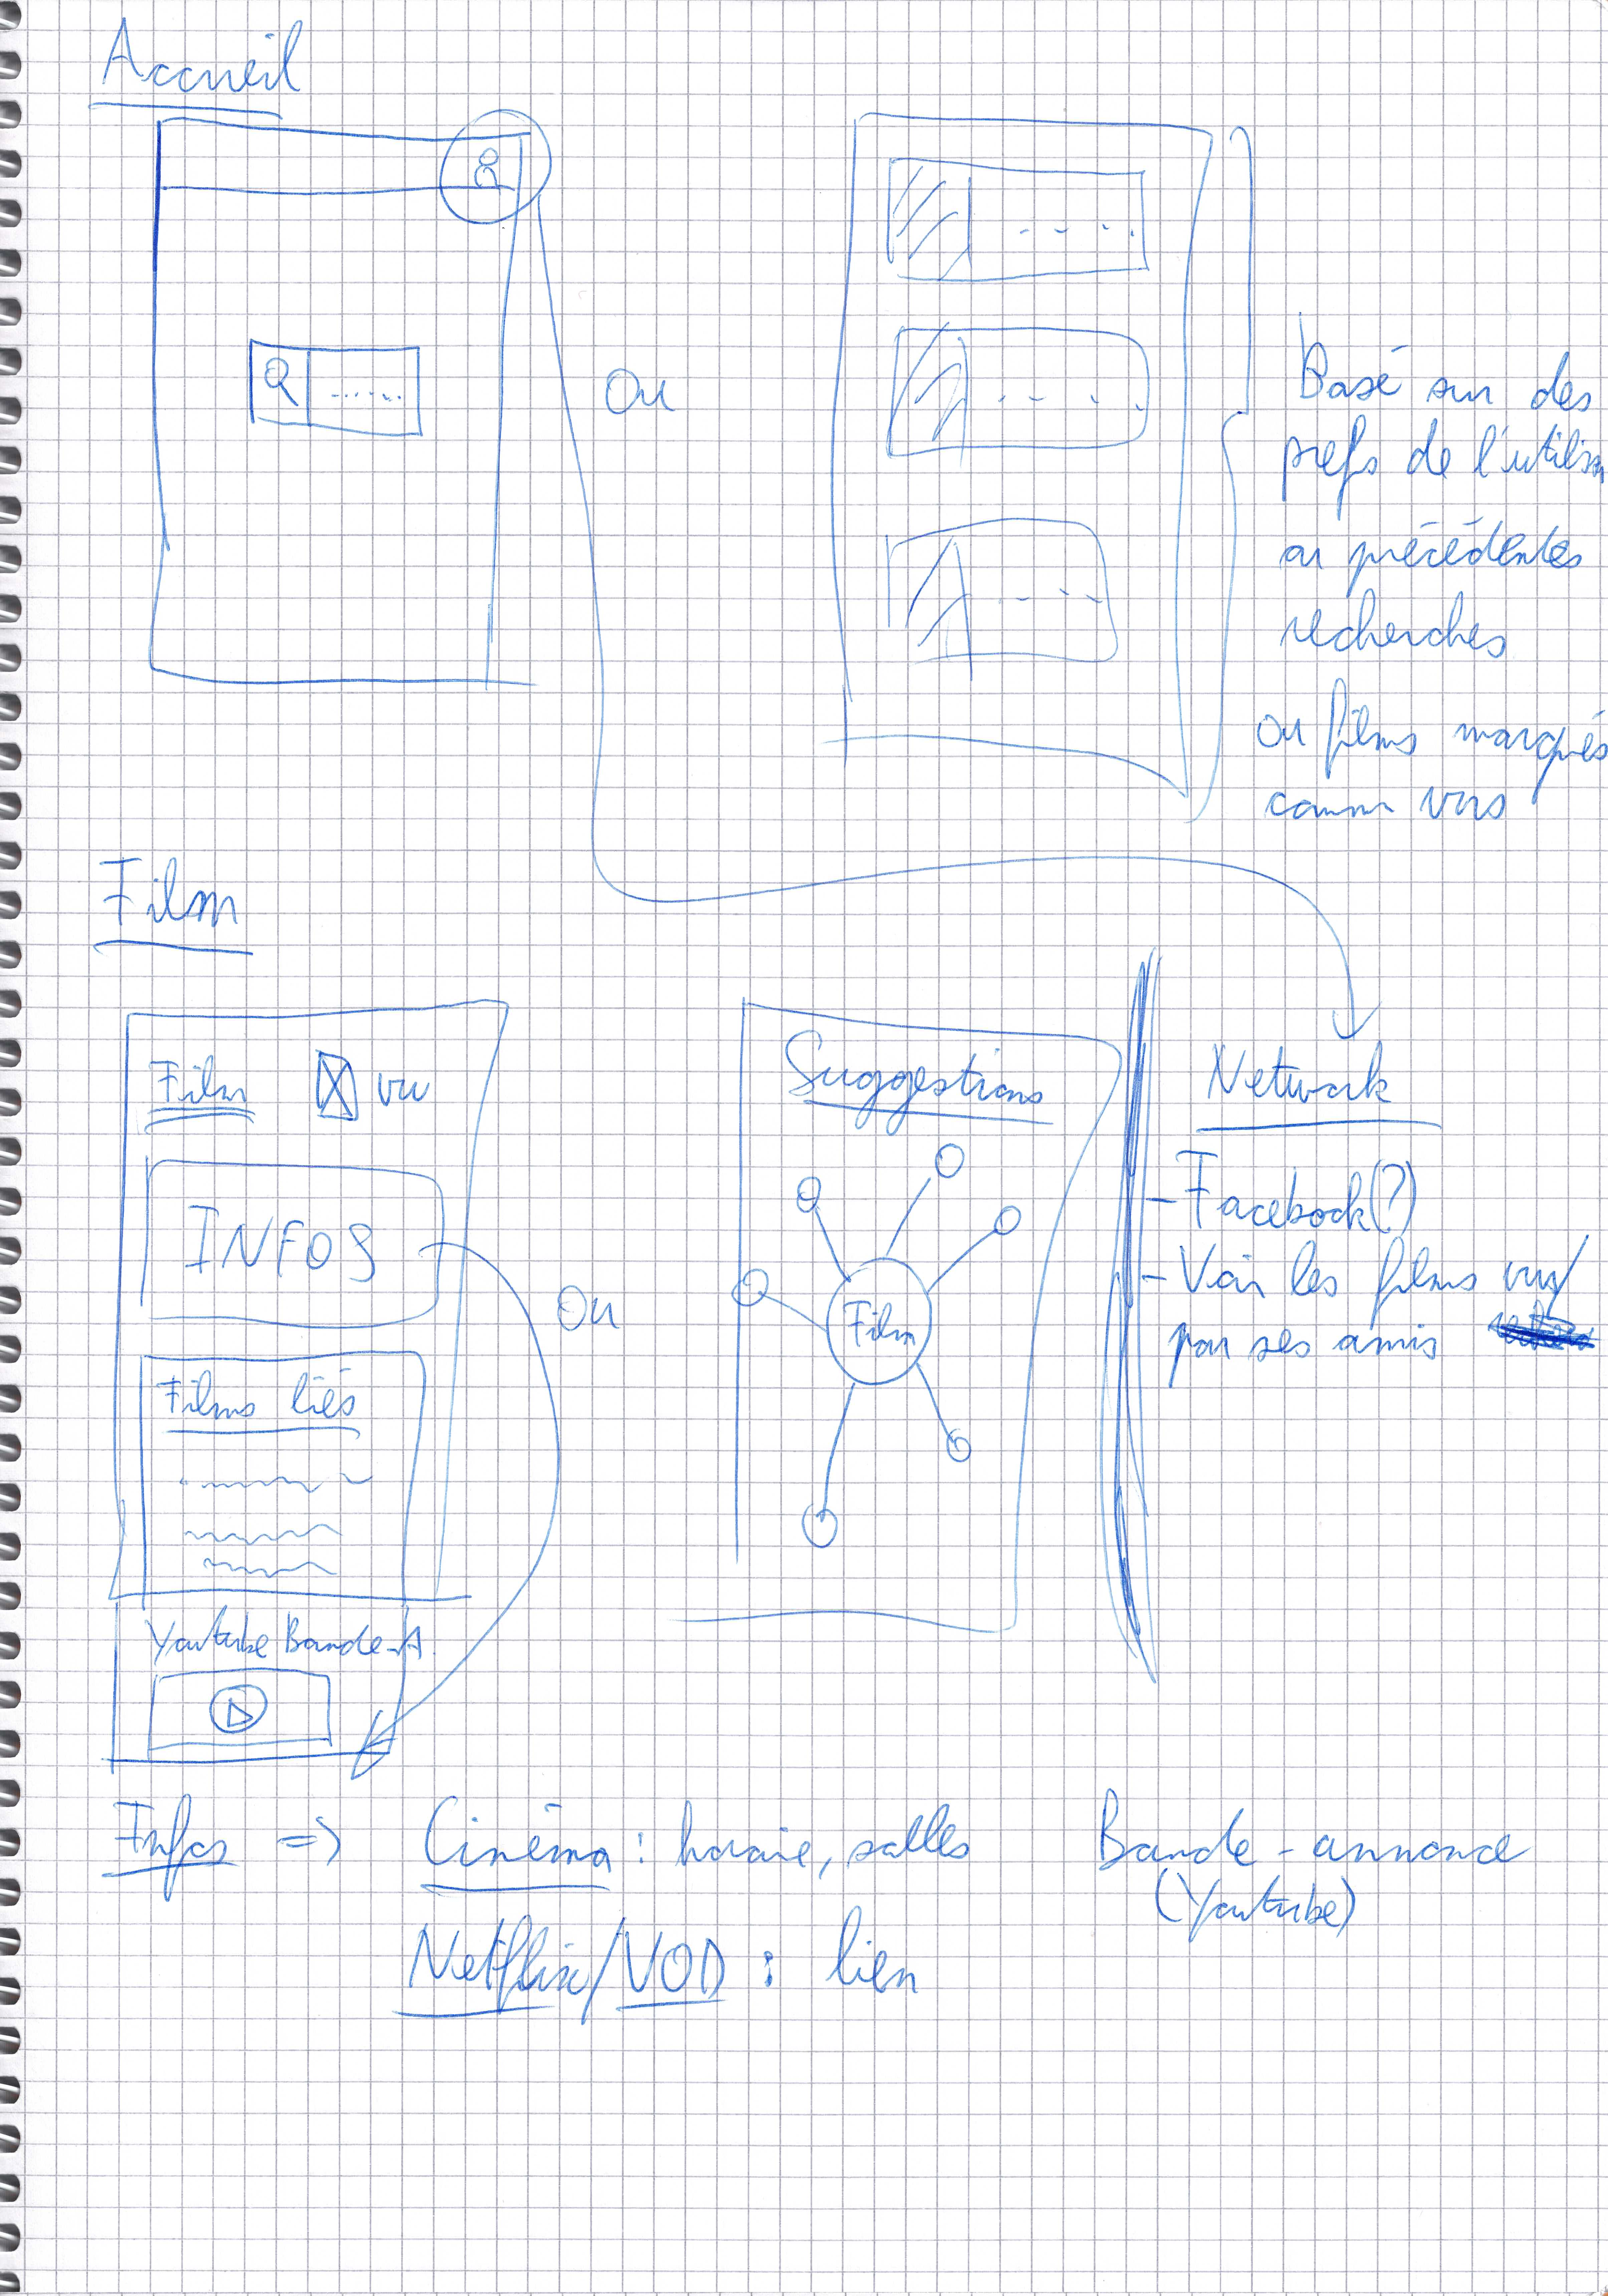
\includegraphics[width=0.8\textwidth]{img/maquettes.jpg}
    \end{center}
    \caption{Maquettes à main levée des vue de l'application}
    \label{maquettes}
\end{figure}

\subsection{Recherche}
Une interface de recherche est mise à disposition. La recherche peut être lancée parmi les films, les acteurs ou les autres utilisateur de l'application selon le choix de l'utilisateur (bouton "radio" ou mécanisme similaire).
Les résultats de la recherche seront présentés sous forme de liste, présentant les différentes actions selon le type de recherche qui aura été effectué :
\begin{itemize}
    \item Si l'utilisateur cherche un film, il obtiendra la liste des films qui correspondent aux critères entrés dans le champs texte de recherche.
    \item S'il cherche un acteur, il obtiendra une liste d'acteurs avec la possibilité de cliquer dessus (comme pour les films) afin d'afficher plus de détails à leur sujet.
    \item S'il cherche un autre utilisateur, il aura alors la possibilité de le suivre en l'ajoutant à son réseau d'amis.
\end{itemize}

\subsection{"Peoples"}
Au même titre que la liste des films tendance, nous avons une interface proposant la liste des acteurs actuellement populaires avec la possibilité de cliquer sur chacun d'entre eux afin d'obtenir plus d'informations à leur sujet.

\subsection{Détails d'un "people"}
Comme pour les détails d'un film, nous avons également une vue présentant les détails d'un acteur, elle permet de consulter diverses informations, telles que sa biographie personnelle et la liste des films dans lesquels il a joué.

\subsection{Mes films}\label{mes-films}
Si l'utilisateur possède un compte dans l'application, il pourra retrouver sa liste de films appréciés ou non, sous une forme similaire à la liste des films tendance (sous-section \ref{films-tendance}).

\subsection{Réseau d'amis}\label{reseau-amis}
La vue réseau d'amis est disponible uniquement si l'utilisateur détient un compte. Son réseau d'amis sera constitué d'une liste d'utilisateurs le suivant (ses "\textit{followers}") ainsi que d'une liste d'utilisateurs auxquels il est abonné (ses "\textit{following}").

\subsection{Authentification}
Au sein de l'application, l'authentification est requise pour consulter certaines vues spécifiques, comme le réseau d'amis (\ref{reseau-amis}) ou les films préférés (\ref{mes-films}) et les vues comprenant des éventuelles informations persistées.
Les autres vues de l'application ne requièrent aucune authentificaion. Ce principe a été mis en place afin de ne pas reproduire un des principaux points faibles des applications actuelles qui est de forcer l'utilisateur à s'authentifier sous peine de ne pas pouvoir utiliser l'application. Notre application demandera à l'utilisateur de s'authentifier uniquement lorsque cela est nécessaire.
 
\subsubsection{Connexion}
La vue connexion comporte simplement deux champs permettant de renseigner le pseudo et le mot de passe afin de s'authentifier.

\subsubsection{Enregistrement}
Cette vue comporte les champs nécessaires à la création d'un compte, à savoir un pseudo (unique), un email et un mot de passe.

\subsection{Navigation}
Pour naviguer d'une vue à une autre, l'utilisateur dispose de différents mécanismes.

\subsubsection{Tabs de navigation}
En bas de l'écran, nous retrouvons une liste de \textit{tabs} (onglets) permettant de naviguer entre les différentes vues de l'application.

\subsubsection{Barre de navigation}
En haut de l'écran se trouve une barre comportant le nom de la vue courrante, un bouton "home" (\ref{films-tendance}) et un contrôle faisant apparaitre le menu latéral.

\subsubsection{Menu latéral}
Finalement, nous avons un menu latéral qui apparaît de gauche à droite de l'écran. Ce menu permet d'afficher les informations relatives au profil de l'utilisateur courant. D'autre part, il propose les action de connexion, création de compte et déconnexion. Si l'utilisateur est connecté, il pourra aussi naviguer vers les vues des films aimés et du réseau d'amis.
